\chapter{The RoFI platform}\label{chap:rofi}

The RoFI platform is expected to allow construction of reconfigurable robotic
systems using small autonomous units. A typical use case for the platform is to
validate algorithms for reconfigurable robots in a physical world or test
hypothesis rather than solving real-world problems.

\section{Design Goals}\label{sec:design_goals}

Our overall goal can be broken down into the following requirements
specification of the platform:

\emph{Platform Requirements}: We expect the platform to define standardized
autonomous modules, which can physically connect via a docking system in
versatile self-reconfigurable systems. The requirements boil down to a design of
module shape and dock positions such that the system can be easily reconfigured.
Versatility can also be supported by the extensibility of the platform -- the
platform should allow for specialized modules (special actuation or sensors).
The platform should allow distributed control as a distributed environment can
be easily converted a central control. However, the vise-versa is not easily
possible.

\emph{Docking System Requirements}: The docking system is a crucial part of the
platform as the modularity relies on it. The dock should allow the modules to
connect in a variety of useful arrangements and should not greatly restrict the
number of possible configurations. Therefore, it should be genderless and should
allow for several possible orientations of two docks. The dock should be also
strong enough to support large systems of modules. To support fault-tolerance of
the platform, disconnection of a module from the mating side should be possible
without the cooperation of the mating side. Such functionality is useful in case
of module malfunction. The docks should also drain energy only when changing
state from locked to unlocked and vice-versa. The dock should also allow for
communication and power sharing among the modules.

\emph{Usability Requirements}: We expect the platform to allow for fast software
development. Therefore, the platform should provide a formal model of the
platform and allow for easy porting of existing algorithms and libraries. The
formal model of the platform allows to reason about systems and also establishes
terminology. Porting existing libraries and algorithms is beneficial for fast
development since it enables to adapt existing, tested code. Both easy
development of new programs and porting existing ones can be achieved by
leveraging of standard technologies. The platform should also provide an
automatic way of program distribution among the modules and should deal with
debugging in the distributed environment to make development for the platform
more pleasant.

\section{The RoFI Platform }

The RoFI platform is a lattice type modular, self-reconfigurable and metamorphic
platform. The platform is defined by:
\begin{enumerate}
    \item a grid system with a module shape requirements (section \ref{sec:aware}),
    \item a docking system (section \ref{sec:dock}),
    \item an inter-module communication (section \ref{sec:communication}) and
    \item module descriptions (section \ref{sec:capabilities}).
\end{enumerate}

The platform also comes with a formalism for describing configurations of
systems built in the platform (section \ref{sec:configuration}) and also gives
an example of a module fulfilling the specification in the form of the
\emph{universal module} (chapter \ref{chap:universal_module}).

\section{Module Shape}\label{sec:aware}

The shape of modules in the RoFI platform is based on a 10cm cube grid. There is
an inscribed sphere in each cell of the grid. By saying a module \emph{occupies
a grid cell} we mean that it occupies the sphere inscribed to the cell. Two grid
cells are adjacent if they share a common face. Therefore, each cell has 6
adjacent cells.

Each module in its default state (with all joints in neutral
position\footnote{Definition of joint follows in the text.}) should occupy one
or more adjacent cells of the grid. If the module occupies more than a single
cell, it is also allowed to occupy the space of corresponding \emph{module
hull}. Consider two adjacent cells occupied by the body. Then there is a convex
hull of their inscribed spheres (see double cell module in figure
\ref{fig:rofi_shapes}). The module hull is then defined as the union of all such
existing convex hulls for the module. See figure \ref{fig:rofi_shapes} for an
example. When we reference a module shape, we use following terminology:
\begin{enumerate*}
    \item \emph{shoe} is a part of the module occupying a cell sphere and
    \item \emph{body} is a part of the module occupying mainly rest space from
    the module hull.
\end{enumerate*}
See figure \ref{fig:um_body_parts} for an example of such naming on the
universal module.

\begin{figure}[!ht]
    \centering
    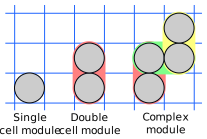
\includegraphics[width=0.7\textwidth]{figures/rofi_shapes.pdf}
    \caption{Example of a module hull construction. Each convex hull of adjacent
    cells is denoted by a coloured area. The module hull is the union of coloured
    ares. Note that the coloured areas slightly overlap the grid. This is only
    for the purpose of visualizations. In reality they fit exactly in the grid.}
    \label{fig:rofi_shapes}
\end{figure}

The modules are allowed to change their shape by offering several degrees of
freedom in the form of \emph{joints}. Joint is a single rotational or linear
degree of freedom. Intuitively, we can view a module as beads, which can rotate
against each other along the axis of joints. For a simple example of a double
cell module movement see figure \ref{fig:grid_aware}.

The motivation for such a restriction of the shape is a property we call
\emph{grid-awareness}. Consider a simple task for a double cell module: having a
grounded left part of the module, move its right part above the left one. Figure
\ref{fig:grid_aware} illustrates the task. If we consider a module which fits
exactly inside a cube-shaped cell, e.g. an M-TRAN module
\cite{haruhisa_kurokawa_m-tran_2003}, the module occupies extra cells during the
movement (marked by red circles in the figure). Such shape restricts the module
movement in a densely occupied grid. However, if we consider a grid-aware module
(in the example double cell module), it only occupies the least required cells
for the movement and therefore should allow for more efficient reconfiguration
algorithms. The key to grid-awareness is the sphere inscribed in a cell.
Therefore, Roombots\cite{bonardi_locomotion_2012} are not grid-aware even they
shape is a sphere. Their bodies cannot be inscribed in spheres inside grid
cells. Grid-awareness, however, comes at a cost. It requires a retractable
docking mechanism as two neighbouring modules can feature only point contact. We
further discuss this in section \ref{sec:dock} and section
\ref{sec:dock_in_grid}, we define allowed positions for docks on a module.

\begin{figure}[!t]
    \centering
    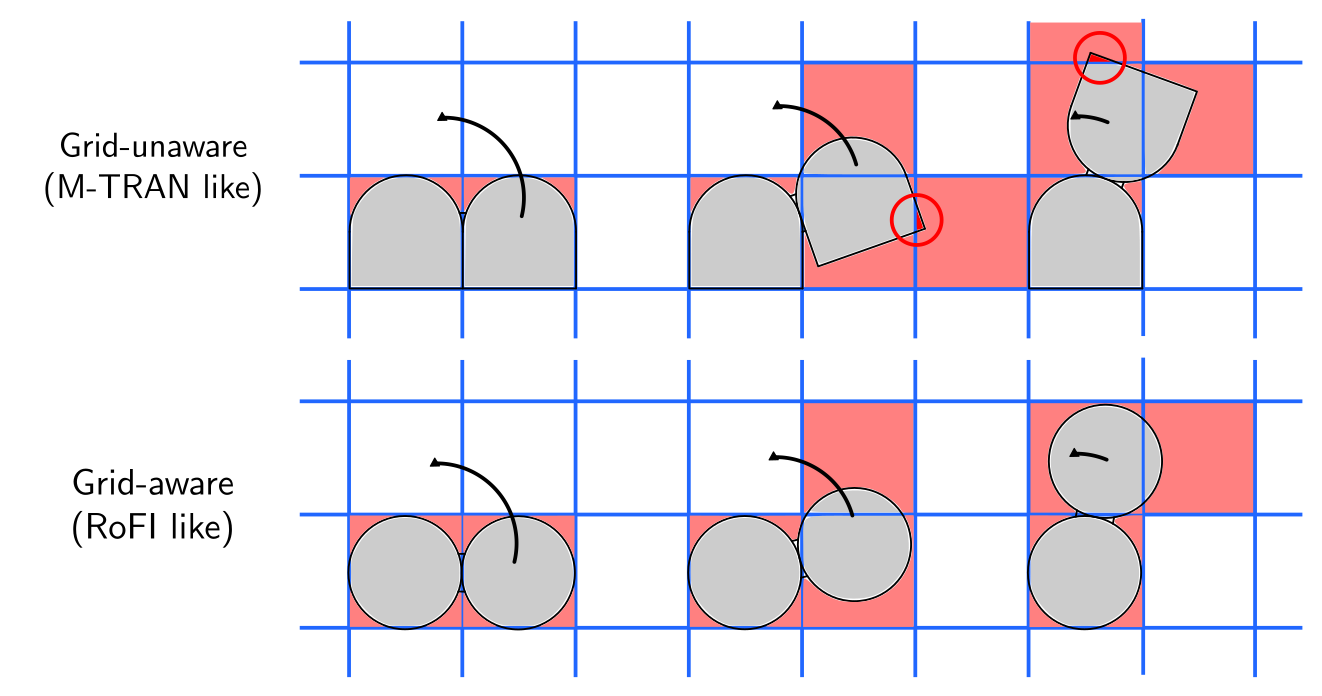
\includegraphics[width=\textwidth]{figures/grid_aware.pdf}
    \caption{Visualization of grid-awareness. Consider two module shapes -- an
    M-TRAN\cite{haruhisa_kurokawa_m-tran_2003} like (int the top row) and a RoFI
    like (in the bottom row). Given the task to move right body over the left
    one, M-TRAN like module occupies extra cells due to small parts of it body
    overlapping out of the gird. On the other hand, RoFI like module occupies
    the least cells required to make the movement. }
    \label{fig:grid_aware}
\end{figure}

We want to point out that even we referred all examples to grid-fitting
positions of the robots (where all movement is performed by steps of
$90^\circ$), we do not give any restriction on the granularity of the movement.
We assume the modules are physically able to move with practically
unlimited granularity (considering limits of a mechanic construction). However,
the reconfiguration algorithms built on top of the system can take only
discrete steps in the movement into account if they need to.

The shape specification allows us to define modules with various shape and
functionality. However, we do not expect the platform to feature many different
types of modules and especially oddly shaped ones. We firmly believe that the
double cell universal module (described in chapter \ref{chap:universal_module}),
should be the primary building block of RoFI systems. However, in future, we
consider having, for example, a passive module (built only from a mechanical
construction), accumulator module or single-cell modules featuring specialized
sensors (e.g., camera) or actuators (e.g., robotic hand or a wheel).

\section{RoFI Docking System}\label{sec:dock}

Since the modules in the RoFI platform are grid-aware, we cannot adapt existing
docking systems from systems like Roombots \cite{bonardi_locomotion_2012} or
M-TRAN III \cite{kurokawa_distributed_2008}. The reason is that two adjacent
modules in the grid feature only a single point contact and not a whole face
contact as it is common in other modular robotic platforms. There is a need for
a retractable dock (see \ref{fig:rofi_locking_example}).

\begin{figure}[t]
    \centering
    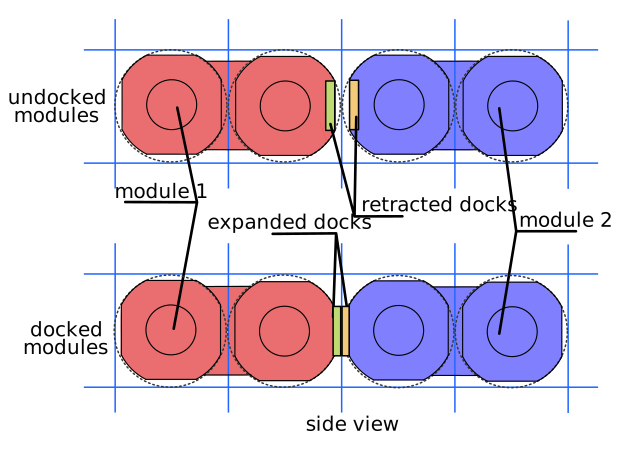
\includegraphics[width=\textwidth]{figures/rofi_locking_example.pdf}
    \caption{Docking procedure. There is a by-default retracted docking system
    in the module which expands when the docking should be performed.}
    \label{fig:rofi_locking_example}
\end{figure}


\begin{figure}[t]
    \centering
    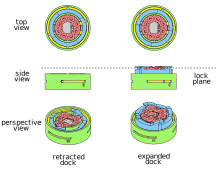
\includegraphics[width=\textwidth]{figures/dock_overview.pdf}
    \caption{The dock from the RoFI docking system. The model is simplified.}
    \label{fig:dock_overview}
\end{figure}

To overcome this issue, we present the RoFI docking system (figure
\ref{fig:dock_overview}). This system is inspired by the HiGen docking
system \cite{parrott_higen:_2014}. In summary, our dock:
\begin{itemize}
    \item allows for connection of two modules when they are not touching side
    by side,
    \item allows for connection in four different orientations,
    \item is genderless (each two docks can connect),
    \item it is based on a mechanical connection (and therefore it is not
    limited by a magnetic force and drains energy only during docking and
    undocking),
    \item can disconnect without participation of the mating side (which also
    allows for connection to a passive dock -- similar to Roombots
    \cite{bonardi_locomotion_2012}) and
    \item supports data communication and power sharing.
\end{itemize}

The docking system is designed to be a stand-alone unit, which can be mass
produced and reused in all modules. It defines a communication interface between
two docks (described in section \ref{sec:dock_interaction}) and communication
interface between module control unit and the dock (described in
\ref{sec:dock_interface}).

\subsection{The Principle of Operation}

The main principle of operation is the same as the principle of the HiGen dock.
There are two key components -- clip and skirt (figure
\ref{fig:dock_key_components}). The clip features four hooks. These hooks can
slide under hooks of the clip from the mating side and form a connection which
prevents pulling the docks apart. When two skirts touch each other, they stop
the two mating docks from rotating against each other. By combining these two
types of joints, we obtain a firm connection between the two docks.

The operation of a single dock is straightforward -- see figures
\ref{fig:dock_overview} and \ref{fig:dock_description}. Consider a dock in the
retracted position. When the shaft ring (yellow) starts to rotate, it translates
the motion to the clip (blue). There is a helical slot in the dock body (see
figure \ref{fig:dock_key_components}) which forces the clip to move upwards (to
``unscrew''). As the clip moves upwards, it carries the skirt. The skirt moves
in a slot which prevents it from rotating against the body and therefore it only
slides upwards. So far, the clip extends to a locking distance. However, the
hooks of the docks could not slide under each other. A horizontal part ends the
helical slot (see figure \ref{fig:dock_key_components}). This ending allows for
sliding the hooks under each other. The pressure on the hooks and skirts causes
force only in the Z direction; there is no need to hold the components in
position by an active element (e.g., motor) and therefore energy is only
required to change state.

\begin{figure}[t]
    \centering
    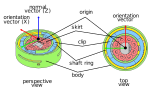
\includegraphics[width=\textwidth]{figures/dock_description.pdf}
    \caption{Naming of the components of the dock. The orientation and the
    normal vector are important for specifying orientation of two connected
    docks. }
    \label{fig:dock_description}
\end{figure}

\begin{figure}[t]
    \centering
    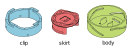
\includegraphics[width=\textwidth]{figures/dock_key_components.pdf}
    \caption{View of the three key components of the dock: clip, skirt and body.}
    \label{fig:dock_key_components}
\end{figure}

See figure \ref{fig:dock_locking_process} for an example of an interaction of
two docks. Situation 1 shows the docks in a position they are in two adjacent
grid cells. By rotation of the shaft ring, the clips and skirts extend
(situation 2). Situation 3 shows fully expended clips and skirts. The skirts are
now connected, and no rotational movement of the docks is possible. The clips
are also at the end of the helical slot. By further rotation of the shaft ring,
the hooks slide under each other and finish the locking process (situation 4).

\begin{figure}[!ht]
    \centering
    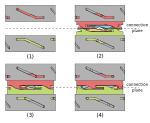
\includegraphics[width=\textwidth]{figures/locking_process.pdf}
    \caption{Illustration of connection of two dock. Clip of the upper dock is
    shown red, skirt of the upper dock is shown blue, clip of the bottom dock is
    shown is as green, skirt of the bottom dock is shown yellow.  Situation 1 is
    the retracted state. The dock pass by the lock plane (2), then continue
    expansion (3) and finish by purely rotational movement(4). }
    \label{fig:dock_locking_process}
\end{figure}

There are two crucial observation to note:
\begin{enumerate*}
    \item the docks are symmetric; therefore there are 4 different orientation
    the docks can lock in;
    \item the movement of two docks does not have to be synchronized, and
    therefore, it is possible for a dock to wait in expanded position or to
    disconnect when the mating module stops responding. The absence of necessity
    for synchronization can also be leveraged for the construction of passive
    docks. The passive dock is a component with no moving parts in a shape of
    an extended dock.
\end{enumerate*}

The symmetry of the dock is best shown on the skirt -- see figure
\ref{fig:dock_skirt_symmetry}. There are four identical blocks on the skirt
along the horizontal and vertical axis. The blocks allows for four different
orientation of the docks. When two skirts are facing, there is a mapping of
blocks from one skirt to the other one. The facing blocks have the property that
the green circle is always facing a red one. This feature is vital for
three reasons:
\begin{itemize}
    \item There are pins on the skirt, which prevents the skirt from
    rotation against another skirt (see perspective view in figure
    \ref{fig:dock_key_components}).
    \item Also, there are magnets in the holes (red -- north facing up, green --
    south facing up) which attract the skirts to each other. The magnets help
    misaligned docks to connect correctly.
    \item By mounting spring contacts in the symmetry blocks, we can build power
    and data transmission lines between modules -- see section
    \ref{sec:dock_interaction} for detailed description.
\end{itemize}
The idea behind symmetry of the clip is the same as the idea behind the skirt
symmetry.

\begin{figure}[!ht]
    \centering
    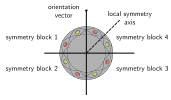
\includegraphics[width=0.8\textwidth]{figures/skirt_symmetry.pdf}
    \caption{Illustration of the skirt symmetry.}
    \label{fig:dock_skirt_symmetry}
\end{figure}

\subsection{Dock Mechanical Implementation}

We designed the dock to be compatible with the 10cm grid. Therefore the dock is
cylindrical, measuring 45~mm in diameter with a depth of 15~mm and can expand up
to 6~mm (module face-to-face distance 12~mm). Compared to the HiGen dock, we
feature less than half the depth (HiGen depth is 32~mm) while preserving the
same docking distance. The thin profile was achieved by swapping positions of
the clip and skirt -- in our case, the clip is the outer ring and skirt is the
inner ring, in the HiGen case skirt is the outer ring and clip is the internal
one. The swap allowed for placing the motor flat (figure
\ref{fig:dock_internal_arrangement}) and therefore, flatter profile of the dock
was achieved. Flat dock profile is a significant advantage -- the inside of the
body can be larger compared to a non-flat profile.

Note that the depth is independent on the diameter. The diameter choices is a
trade-off between connection stability (increases with diameter) and module size
(also increases with diameter) as we explain in section \ref{sec:dock_in_grid}.
We designed our model to be parametric -- it is possible to specify desired
diameter, connection distance and material thickness, and generate a new model.
The depth of the dock $h$ is equal to $h=l+6w$, where $l$ is the connection
distance (in our model 6~mm) and $w$ is wall thickness (in our model 1.5~mm).
Note that the parameters for the model cannot be chosen arbitrarily as there
some limitation (e.g., motor size).

The dock composes of 5 custom components:
\begin{enumerate*}
    \item body,
    \item shaft ring,
    \item clip,
    \item skirt and
    \item motor mount.
\end{enumerate*}
These parts are for prototyping 3D printed from the PLA material, however, the
components could be after few modifications lathed and milled from metal. We
build this assumption on a similar component complexity as the ModRED docking
system \cite{hossain_towards_2014}. The authors show modifications necessary to
achieve serial manufacturability. The motor used in the design is commonly
available ``Pololu 298:1 Micro Metal Gearmotor HPCB
6V''\footnote{\url{https://www.pololu.com/product/3069}}.

Rather than providing technical drawings of the individual components, we
provide a CAD model in Fusion 360. The model can be found in the Fusion Cloud:
\url{https://a360.co/2pIQzZ3}.

As we mentioned, the dock is supposed to be a reusable stand-alone unit.
Therefore, there is a PCB with driver electronics in the back of the dock.
However, current prototype does not feature it. The purpose of the electronics
is to:
\begin{enumerate*}
    \item drive the motor in the clip,
    \item buffer incoming communication from an attached dock,
    \item provide a bus interface for a master controller in the module to
    easily control the dock, and
    \item provide an interface for power sharing.
\end{enumerate*}
The electronics is supposed to be rather simple -- small microcontroller is
supposed to drive H-bridge for the motor, detect the limit position of the
mechanism via hall sensors and appropriately placed magnets. Usage of hall
sensors instead of mechanical switches allows for further minimization compared
to the HiGen dock.

\begin{figure}[!ht]
    \centering
    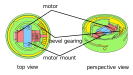
\includegraphics[width=\textwidth]{figures/dock_arrangement.pdf}
    \caption{Internal arrangement of the components inside the dock. Note that
    skirt and clip are not shown. The skirt and clip are swapped compared to the
    HiGen dock. This with a bevel gearing allow for placing the motor flat and
    therefore achieving half the depth of dock.}
    \label{fig:dock_internal_arrangement}
\end{figure}

\subsection{Mutual Orientation of the Docks}\label{sec:mutual_orientation}

To be able to describe system made out of modules in section
\ref{sec:configuration} we define the \emph{mutual orientation} of the docks. As
shown in figure \ref{fig:dock_description}, there is an orientation vector on
the dock. When two docks connect, there can be an angle of $0^\circ$,
$90^\circ$, $180^\circ$ or $270^\circ$ between their orientation vectors
(measured counterclockwise from a perspective one of the modules from shoe
center to the dock center). Notice, that the angle is the same no matter which
module we choose. Therefore, we give a following convention for the mutual
orientation:

If we aim one of the orientation vectors up (to the \emph{north}), the other
vector aims either:
\begin{enumerate*}
    \item \emph{north},
    \item \emph{east},
    \item \emph{south} or
    \item \emph{west}
\end{enumerate*}
as shown in figure \ref{fig:dock_orientation}. Therefore we define the mutual
orientation $o$ to be an element of $\mathcal{O} = \{N, E, S, W\}$.

\begin{figure}[!ht]
    \centering
    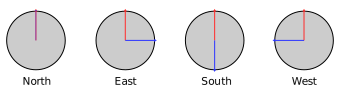
\includegraphics[width=\textwidth]{figures/dock_orientation.pdf}
    \caption{Possible orientation of two docks. Orientation vector of current
    perspective is shown as red, the orientation vector of mating dock is shown
    as blue. Note that during a connection, it does not matter which dock's
    perspective we choose.}
    \label{fig:dock_orientation}
\end{figure}


\subsection{Docks Interaction}\label{sec:dock_interaction}

When to docks are connected, they can exchange binary blobs and share power. The
communication and power sharing is accomplished by mechanical contact using pogo
pins placed in the inner part of the skirt. The communication between two docks
is implemented as a simple UART.

To allow docks to connect in four different mutual orientations, we use a
similar pin arrangement as the HiGen dock \cite{parrott_higen:_2014}. Figure
\ref{fig:dock_pins} shows the pin arrangement. The pins are arranged such that
in each orientation one of the pin sections A or B is in contact with one of the
pad sections 1 or 2. There are five pins in total; two pins for power-sharing
(GND and 48 V), two pins for UART (TX and RX) and a dedicated sense pin used for
detection of the mutual orientation. The orientation could be retrieved by
detecting which communication line is active. However, we find such solution
much more complicated. The dedicated sense pin can also easily recognize if the
mating site is still attached.

\begin{figure}[t]
    \centering
    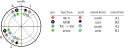
\includegraphics[]{figures/dock_pins.pdf}
    \caption{Pin arrangement on a dock skirt. }
    \label{fig:dock_pins}
\end{figure}

Mutual orientation detection works by permanently pulling sense 1 low and sense
2 high (over a protection resistor) as shown in figure \ref{fig:dock_block}.
Exactly one of the pins sense A and sense B will be either pulled low or pulled
high; the other one will float. The mutual orientation can be determined by the
table in figure \ref{fig:dock_pins}.

The docks communicate over UART with 8 bits, no parity and a 1.5 stop bit at 6
Mbaud/s\footnote{The communication speed is easily achievable due to a short
physical communication distance.}. The words are transmitted in little-endian
byte order. The communication protocol between two docks is simple as the only
allowed operation is to pass one binary blob from one dock to another. The blobs
are wrapped in a frame with the following format:

\bigskip
\begin{bytefield}{32}
    \bitheader{0,7,8,15, 16, 31} \\
    \bitbox{8}{\texttt{0xAA}}
    \bitbox{8}{\textit{reserved}}
    \bitbox{16}{content type} \\
    \bitbox{16}{payload length} & \bitbox[r]{16}{} \\
    \wordbox[lbr]{2}{payload} \\
    \bitbox{32}{CRC}
\end{bytefield}
\medskip

\noindent The frame is transmitted to the mating dock over UART. If the mating
dock is unable to handle the incoming frame or the frame is corrupted (CRC
mismatch), the dock can discard the frame\footnote{This behavior mimics the
Ethernet interface.}. Bytes of the outcoming frame are required to be sent
consequently with no additional delay. There is a silent period of 8 bytes (14
\si{\micro\second}) after each frame. The receiver should discard incomplete
frame after the silent period and prepare for next incoming frame. The hardware
can implement baud rate correction algorithms and leverage the constant header
0xAA for this purpose. The content type field identifies the content in payload
and allows to transmit various protocols over the docks, (e.g., IP datagrams,
RoFI debug messages, RoFI firmware upgrades etc.). The dock is allowed to treat
different content differently (e.g. rearrange them in send buffer, drop them,
etc.).

\begin{figure}[t]
    \centering
    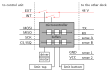
\includegraphics[width=0.9\textwidth]{figures/dock_block.pdf}
    \caption{Block diagram of the dock functionality}
    \label{fig:dock_block}
\end{figure}

\subsection{Dock Power-sharing}

The connection of two docks is direct with no galvanic isolation. Therefore the
modules in the RoFI systems are required to share the same ground potential or
float before the connection is performed. The power is shared on a single 48 V
line. We choose a 48 V line to mitigate the power losses on the conductors.

The dock exposes two power lines to the module -- \emph{EXT} and \emph{INT}. The
EXT line is required to be directly connected to all EXT lines of the other
docks in a module. The purpose of the EXT line is to share power between
connected devices. The INT line is supposed to power the module and, e.g.,
charge an internal accumulator. See example of dock connection in the universal
module in figure \ref{fig:um_internal}. Both of these lines can be connected
to or disconnected from the source independently. The hardware implementation of
the switch is shown in figure \ref{fig:dock_biswitch}. A simple transistor
switch is not enough as the current can flow both directions. The switch also
monitors line voltage and measures current via electromagnetic coupling.

\begin{figure}[t]
    \centering
    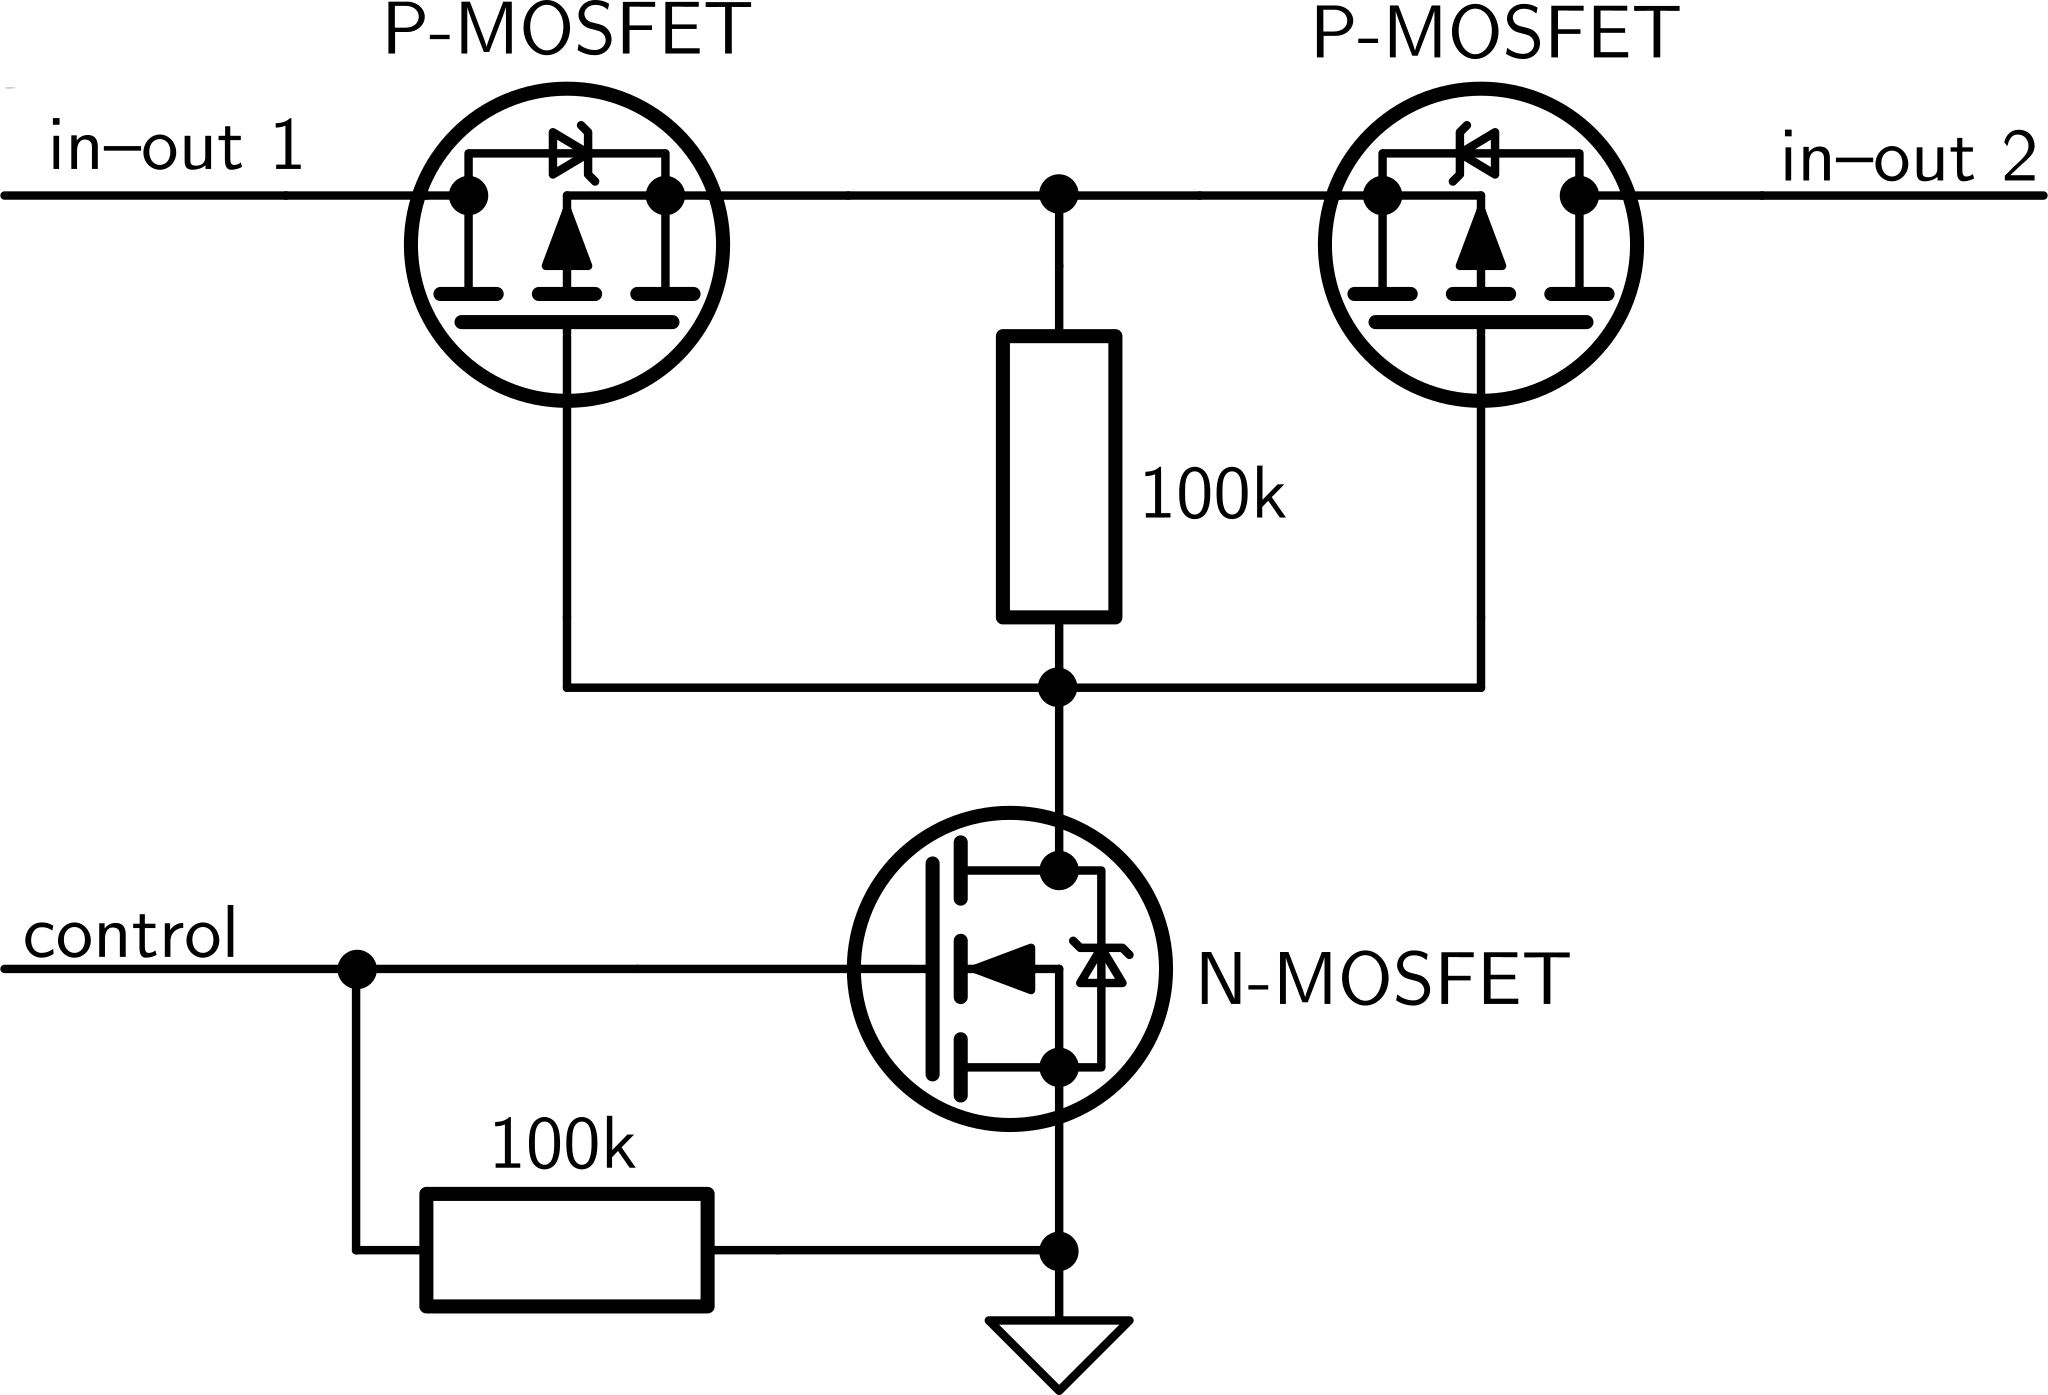
\includegraphics[width=0.7\textwidth]{figures/dock_biswitch.pdf}
    \caption{Implementation of bidirectional switches in the dock.}
    \label{fig:dock_biswitch}
\end{figure}

The separation of the power lines into the EXT and INT lines allow for
different modes of operation:
\begin{enumerate}
    \item The module does not participate in power-sharing (all switches are
    opened). The module serves as an isolator and can be used to separate
    the system into several independent power-sharing components.
    \item The module connects the docks to the EXT line. The module servers a
    power bridge, but does not drain nor source any power to the system.
    \item One or more docs are connected to the INT line. The module can drain
    power from or source power to the system.
    \item The previous modes are combined -- e.g., two docks are connected to the
    EXT line and therefore, can share power, but the module is connected to
    another dock.
\end{enumerate}

The RoFI modules are expected not to share power by default. The power sharing
mechanism should not by default connect all the modules in a system. The modules
should run on their own accumulator and only if a module in the module requires
external power, the circuit from the EXT lines should be established and the
energy should be transferred.

\subsection{Dock Interface}\label{sec:dock_interface}

The docks in a module should be controlled by the module control unit. There are
usually multiple docks in a single module.

The dock provides SPI slave interface on 3.3 \si{\volt} level to control the
dock (figure \ref{fig:dock_block}). The chip select pin (CS) also serves as an
interrupt to the master -- when an interrupt is issued, the pin is pulled low by
the slave. Words are transmitted in the little-endian byte order, bytes are sent
most-significant bit first. The data are read at the rising edge of the clock
signal. The dock should support at least 10 \si{\mega\hertz} clock signal.

There can be multiple variants of the docks (e.g., variants featuring sensors).
There is unique number identifier assigned to each dock variant. So far, we
specify only dock variant 1 with no sensors, further referenced as a \emph{base
dock}. The following text describes revision 1 of the communication protocol.
Future revisions might be released, but they must be backward-compatible.

The communication on the bus is performed in transactions -- each transaction
starts by master pulling CS low and end by releasing CS back to high. Incomplete
transactions must have no observable effect. Each transaction follows the format:

\bigskip
\begin{bytefield}{32}
    \bitheader{0,7,8} \\
    \bitbox{8}{command} & \bitbox{24}{command data} \\
    \wordbox[tb]{2}{pause at least 8 bytes (no clock)}  \\
    \wordbox{2}{dock response}
\end{bytefield}

\noindent No padding of the command data or dock response is required. The
commands 0--127 are reserved for the base dock, and all dock types are required
to support them. The commands 128-255 are dock type specific. The basic commands
are:

\paragraph{Version command (0):} has no command data. The response is in the
format:

\bigskip
\begin{bytefield}[bitwidth=1.75em]{16}
    \bitheader{0, 15} \\
    \bitbox{16}{dock variant} \\
    \bitbox{16}{protocol revision}
\end{bytefield}

\paragraph{Status command (1):} can be used to query dock status and issue
status changing commands like expanding or retracting the dock. We consider
following bitfields for this command:
\begin{itemize}
    \item P (position, 1-bit) -- 1: expanded dock, 0: retracted dock,
    \item I (internal, 1-bit) -- 1: the INT line is connected, 0: the line is disconnected,
    \item E (external, 1-bit) -- 1: the EXT line is connected, 0: the line is disconnected,
    \item C (connected, 1-bit) -- 1: the dock is connected (the sense pin is
    active), 0: the dock is disconnected and
    \item O (mutual orientation, 2-bit) -- 0: north, 1: east, 3: south, 4: west.
\end{itemize}

The command data consist of two part: a status bitmask and a write mask. By
setting a corresponding bit in write mask, we can change the state of the
corresponding feature of the dock to the state specified by a status bitmask.
E.g., by setting bit I to 1 and setting corresponding bit in write mask, the INT
line will be connected. Zero bits in the write bitmask are left unchanged. The
format of the command data is:

\bigskip
\begin{bytefield}[bitwidth=1.75em]{16}
    \bitheader{0-15} \\
    \bitbox{1}{P} &
    \bitbox{1}{I} &
    \bitbox{1}{E} &
    \bitbox{13}{\textit{reserved}} \\
    \bitbox{3}{write mask} &
    \bitbox{13}{\textit{reserved}}
\end{bytefield}

\noindent The dock response follows the similar format as the command. The dock
returns the status before performing the command. It also sends the count of
blobs waiting in the buffer for transmission, count of blobs not retrieved by
the master and voltage and current on the power lines. The voltage in 8.8
fixed-point number in volts, the current is in 8.8 fixed-point number in
Amperes. The format is following:

\bigskip
\begin{bytefield}[bitwidth=1.75em]{16}
    \bitheader{0-15} \\
    \bitbox{1}{P} &
    \bitbox{1}{I} &
    \bitbox{1}{E} &
    \bitbox{5}{\textit{resserved}} &
    \bitbox{1}{C} &
    \bitbox{2}{O}
    \bitbox{5}{\textit{reserved}}\\
    \bitbox{8}{blobs pending to send} & \bitbox{8}{blobs pending to retrieve} \\
    \bitbox{16}{INT line voltage (8.8 fixed-point)} \\
    \bitbox{16}{INT line current (8.8 fixed-point)} \\
    \bitbox{16}{EXT line voltage (8.8 fixed-point)} \\
    \bitbox{16}{EXT line current (8.8 fixed-point)}
\end{bytefield}

\paragraph{Interrupt command (2):} can be used to query interrupt reason and to
enable and disable interrupts. There are following interrupts:

\begin{itemize}
    \item C -- connect or disconnect event occurred (the sense pin change) and
    \item I -- new binary blob received.
\end{itemize}
The data command is a bitmask with enabled interrupts:

\bigskip
\begin{bytefield}[bitwidth=1.75em]{16}
    \bitheader{0-15} \\
    \bitbox{1}{C} &
    \bitbox{1}{I} &
    \bitbox{14}{\textit{resserved}}
\end{bytefield}

\noindent The response follows the same format:

\bigskip
\begin{bytefield}[bitwidth=1.75em]{16}
    \bitheader{0-15} \\
    \bitbox{1}{C} &
    \bitbox{1}{I} &
    \bitbox{14}{\textit{resserved}}
\end{bytefield}

\noindent Bits set to 1 signal interrupt reason. After the response is sent, all
interrupt reasons are cleared. Therefore, the mask returns all interrupts
reasons from the last query.

\paragraph{Send blob (3)} is used to send a binary blob. The command data are
formatted as follows:

\bigskip
\begin{bytefield}[bitwidth=1.75em]{16}
    \bitheader{0, 15} \\
    \bitbox{16}{content type} \\
    \bitbox{16}{blob length} \\
    \wordbox{2}{blob data}
\end{bytefield}

\noindent The size of a blob should be less than 1500 bytes (to be compatible
with Ethernet). However, the dock might supporter larger blobs.

The response follows the format:

\bigskip
\begin{bytefield}[bitwidth=1.75em]{16}
    \bitheader{0-15} \\
    \bitbox{8}{akcnowledgment}
\end{bytefield}

\noindent The acknowledgment is nonzero if the dock was able to place the blob
in its transmission buffer. However, the blob can be still rejected by the
mating dock.

\paragraph{Receive blob (4)} is used to obtain a received blob from the mating
dock. The oldest received blob is sent. The command has no data. The response
follows the format:

\bigskip
\begin{bytefield}[bitwidth=1.75em]{16}
    \bitheader{0, 15} \\
    \bitbox{16}{content type} \\
    \bitbox{16}{blob length} \\
    \wordbox{2}{blob data}
\end{bytefield}

\noindent If there are no pending blobs, a blob of zero length is returned.

\subsection{Docks in the Grid System}\label{sec:dock_in_grid}

The shape requirements in section \ref{sec:aware} omitted the placement of the
docks. As we have already defined the RoFI in this section, we can complete the
shape requirements with possible dock placements.

Consider a shoe, the basic abstract building block of modules (figure
\ref{fig:dock_positions}). We define the origin of the shoe in the middle of the
sphere. There are up to 6 adjacent shoes in the grid (in both direction of all
axis X, Y, and Z.) The directions define six possible dock positions which we
name after an axe direction. We name it $\mathcal{P} = \left\{+X, -X, +Y, -Y,
+Z, -Z\right\}$. We also give an orientation of the dock (see figure
\ref{fig:dock_positions}).

Therefore, each RoFI module can specify a subset of docks it features for each
cell it occupies. Once we introduce module descriptors in section
\ref{sec:capabilities}, we will be able to name each dock unambiguously.

\begin{figure}[t]
    \centering
    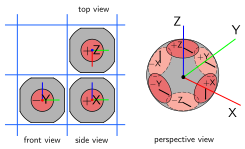
\includegraphics[width=\textwidth]{figures/dock_positions.pdf}
    \caption{Given a shoe the docks are allowed on 6 positions -- in the
    middles of faces of the corresponding cell cube. The docks are named using
    the axis names. Small arrows denote orientation vector of each dock.}
    \label{fig:dock_positions}
\end{figure}

\section{Inter-module Communication}\label{sec:communication}

Inter-module communication is an essential part of a modular robotic system.
Without it, there is no space for emergent behavior to form. There are two
possible means of communication: wireless one and wired one. Both of them
has its advantages and disadvantages.

The wireless communication is easy to implement, as there is no need to
establish a physical connection between the modules. Absence of physical wiring
simplifies docking mechanism and also allows for communication of separate
systems of modules. However, due to its nature, it does not scale well as all
the modules share the same medium and only a single module can transmit at a
time. Also, standard networking technologies like WiFi or Bluetooth are not
suitable for handling possibly hundreds of device in one place, especially in
an embedded environment.

On the other hand, wired communication can scale well as every two connected
modules can communicate without being limited by the other modules. It can also
be more power efficient compared to the wireless one. As there is already a need
for physical connection, a power-sharing interface can be added at minimal cost.
Therefore the connected modules can share and distribute energy. Unlike the
wireless one, there is a need for routing as there is no shared medium and only
adjacent modules can communicate.

The RoFI platform relies primarily on a wired communication between every two
connected modules and optionally allows for wireless communication. This
design choice allows for fast and parallel communication inside a single system
and also allows to establish a communication with a remote system.

With the RoFI platform we do not want to reinvent the wheel and, e.g., come up
with a custom communication and routing protocol based on RS-485 like M-TRAN or
the CAN in case of the HyMod project \cite{parrott_hymod:_2016}. For example,
the CAN bus is fault tolerant and provides prioritized messages, however for
purposes of modular robots, it features several disadvantages:
\begin{itemize}
    \item it has a limited bandwidth of 1 Mb/s \cite{noauthor_road_2013},
    \item it does not scale well as all devices share the same medium,
    \item cannot be cyclic and therefore, needs bus switches to remove cycles,
    \item needs an adjustable impedance based on the topology
    \cite{parrott_hymod:_2016}.
\end{itemize}

Therefore, the RoFI platform leverages traditional computer network based on the
TCP/IP protocol and stack. The TCP/IP protocol allows for seamless operation
with existing computer networks and services. The users can use traditional
sockets, port OpenMPI to their projects or use the network for sending debug
logs from the distributed environment. It potentially open doors for global
communication of the RoFI systems. Using TCP/IP also makes indistinguishable
wired and wireless connection from each other. Routing and robustness also come
for free. The downside of the TCP/IP stack is its complexity; however, this is
partially compensated by the existence of ready-to-use implementation even for
embedded platforms (eg., lwIP \cite{noauthor_lwip_nodate}).

There are two possibilities to implement the TCP/IP in the platform: either use
Ethernet to connect the modules (making each module to act either as a hub or
switch) or introduce a custom L1/L2 layer from the OSI/ISO model
\cite{braden_requirements_1989}. Introduction of custom L1/L2 layers is quite
common (e.g. \cite{lindgren_ip_2008} or \cite{waitzman_ip_1999}).

We have already defined the communication between two docks in the section
\ref{sec:dock}. The dock connection allows us to pass arbitrary packets of data
between two modules. Considering concrete implementation in lwIP, these two
operations, sending a receiving of a packet (possibly with a custom header), is
all that is necessary to implement a custom device driver. A device driver is a
terminology of lwIP and basically is equivalent of the L2 of ISO/OSI model.

There is also no need to implement custom routing nor switching -- each dock
represents a single network interface. There are only up to 2 docks on a single
full-duplex medium; therefore, no switching is required. The routing of IP
packets is handled by the L3 and is usually already implemented in the stack.


\section{RoFI Capabilities}\label{sec:capabilities}

The section \ref{sec:aware} gives an idea about all possible shapes of the RoFI
modules and also provides examples of use cases for shape other than the
universal module. To allow interaction of different modules and also to build
a formal description of RoFI systems, there is a need to establish a way to
describe various modules and their capabilities. There are two aspects to
consider:
\begin{enumerate}
    \item modules have different shapes and can perform different movements and
    \item modules feature different sensors and special functions.
\end{enumerate}

\emph{RoFI descriptors} cover both of these aspects. Descriptors can be
exchanged by the modules when they connect to build a notion of the system which
is essential for any reconfiguration. We distinguish two type of descriptors:
\begin{enumerate*}
    \item \emph{shape descriptor} ($\mathcal{D}_S$) and
    \item \emph{capability descriptor} ($\mathcal{D}_C$).
\end{enumerate*}

We define the shape descriptor $\mathcal{D}_S$ as a tuple $(S, B, E, t, d)$
\begin{itemize}
    \item $S$ is a finite set of shoes,
    \item $B$ is a finite set of bodies,
    \item $E$ is a finite set of edges, formally $E \subset (S\cup B)^2$ such
    that there are no symmetric edges and self-loops,
    \item $t$ is a function returning a transformation function (joint
    transformation matrix) for given edge, formally: $t:
    E\rightarrow(\mathds{R}\rightarrow\mathds{R}^{4\times4})$,
    \item $d$ is a function giving a set of dock present on each shoe. Formally,
    $d: S\rightarrow 2^\mathcal{P}$.
\end{itemize}
Intuitively, $\mathcal{D}_D$ is an oriented graph, with two types of nodes --
shoes and bodies, where edges are labeled by functions returning 3D
transformation matrixes. Note that the graph can be cyclic; however, for each
pair of vertices, there is at most one edge. When drawing descriptors we denote
shoes as circles, bodies as squares and we write the functions on edge. See
an example of such a descriptor for a universal module in figure
\ref{fig:um_descriptor}.

\begin{figure}[t]
    \centering
    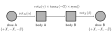
\includegraphics[width=\textwidth]{figures/um_descriptor.pdf}
    \caption{Shape descriptor for an universal module. See figure
    \ref{fig:um_body_parts} and \ref{fig:um_axis} for a visualization of the
    module and its axis. Function $\text{rot}_A(x)$ returns a 3D rotation matrix
    along axe $A$ and $x$ radians, $\text{trans}_A(x)$ returns a 3D translation
    matrix in direction of axe $A$ and distance $x$ units, $\text{sym}$ returns
    a matrix flipping direction of all axis. $G$ denotes size of the grid.}
    \label{fig:um_descriptor}
\end{figure}

Each edge with a non-constant function represents a joint. In the further text
we will abuse the notation a little and name the edges, arguments of the
corresponding transformation functions and corresponding joints by the same name
-- usually by a small Greek letter. The type of the object represented by the
name should be obvious from the context. For example, we name the edge
$(\textsf{shoe A}, \textsf{body A})$ as $\alpha$, the same as the corresponding
joint (figure \ref{fig:um_axis}) and the argument of rotation. Also, for
practical reasons we consider all descriptors to have unique naming of shoes and
bodies (easily achieved by prefixing the name by module name); however, in the
examples, we omit the prefix to make thing simple.

Given the joint positions, the shape descriptors allow for easy computation of
shoe positions in the space. The path in a descriptor between two shoes defines
a transformation matrix representing relative the position of the two shoes.
However, finding such a path might not always be possible due to an orientation
of the edges. By defining a function flip for labeling reversed edges such that:
\[\text{flip}(\text{f})(t) = (\text{f}(t))^{-1}, \text{ for every } t \text{ in
range of a corresponding joint}\] an orientation of an edge can be reversed.
Once reversed, the edge is labeled by a function returning inverse
transformation compared to the original label. Therefore, there is a path
between every two shoes in a module\footnote{The module must be strongly
connected by definition.}.

It is possible to extend the idea of module descriptors further to find
positions of the docks. A descriptor of a single shoe can be constructed in the
same manner a descriptor for any other module (figure
\ref{fig:shoe_descriptor}). The transformations for docks are constant
functions. The coordinate system is transformed such that the axis orientation
is the same as in figure \ref{fig:dock_description} -- the Z axe is
perpendicular to the docks, and the X axe is coincident with the orientation
vector. We do not consider the docks to be a part of the shape descriptor as
they are the same for each shoe and therefore for the sake of simplicity, they
can be omitted. However, we find them useful to consider the following
construction.

\begin{figure}[t]
    \centering
    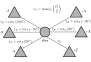
\includegraphics[width=0.8\textwidth]{figures/shoe_descriptor.pdf}
    \caption{Shape descriptor of a shoe. Triangles represent docks. See figure
    \ref{fig:dock_positions} for visualization of physical layout.}
    \label{fig:shoe_descriptor}
\end{figure}

So far, we considered descriptors only in the context of a single module. We can
further extend it to multiple modules. Two descriptors can be joined by adding
edges between connected docks. The relative position of any two shoes in the
system can be computed using this graph. The construction of the connection is
illustrated in figure \ref{fig:connection_descriptor}. We will refer to this
operation as \emph{shape descriptor union}.

\begin{figure}[t]
    \centering
    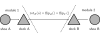
\includegraphics[width=0.8\textwidth]{figures/descriptor_connection.pdf}
    \caption{Illustration of connection of two module descriptors. Each module
    has a shoe (shoe A, shoe B) with docks they connect to each other. To
    connect the modules, new edge is constructed between the docks. Parameter
    $o$ is the mutual orientation of the docks. Note that it does not matter on
    the edge orientation as the mutual orientation is symmetric as shown in
    section \ref{sec:mutual_orientation}. }
    \label{fig:connection_descriptor}
\end{figure}

To allow algorithms take various sensors present on modules in an account,
simple sensor enumeration is not enough as the position of sensor matters.
Therefore, the RoFI platform allows sensors to be placed on faces of the shoe.
The faces are named as the corresponding docks (figure
\ref{fig:dock_positions}). The capability descriptor $\mathcal{D}_C$ is a
function $\mathcal{D}_C: S\times\mathcal{P} \rightarrow 2^{I}$, where $I$ is a
set of all possible sensors. Intuitively, $\mathcal{D}_C$ is a labeling of
individual docks on the module assigning sensors to them. The set of all sensors
$I$ contains sensor-dependent descriptions\footnote{As there exists only the
universal module we consider specification of the sensor format rather
premature.}.

\section{RoFI Configurations} \label{sec:configuration}

So far, we gave means to describe a single module. To ease and unify the
development of a firmware and reconfiguration algorithms, we also give means to
describe a system consisting out of the RoFI modules.

First, there is a globally unique ID (\emph{GUID}) assigned to each instance of
a module. GUID is a 128-bit number to prevent GUID exhaustion. Second, when
talking about RoFI systems, we distinguish two terms:
\begin{enumerate*}
    \item \emph{topology} ($\mathcal{T}$) and
    \item \emph{configuration} ($\mathcal{C}$):
\end{enumerate*}

\paragraph{topology} Intuitively, topology describes the connection between the
modules in a system and does not care about the physical layout of the modules.
Formally, we define a topology $\mathcal{T}$ as a tuple $(M, E, d)$:
\begin{itemize}
    \item M is a finite set of modules represented by GUID, formally $M\subset
    G$, where $G$ is a set of all GUIDs.
    \item E is a finite set of undirected edges (connections) between the
    modules, formally $E\subset M\times M$. Note that the undirected edges
    forces that both modules have to actively participate in a connection.
    \item $d$ is a labeling function for edges. The labels are tuples in form
    $(o, d_a, d_b)$, whrere $o\in\mathcal{O}$ is a mutual orientation of
    connected docks, $d_a$ and $d_b$ from modules in the edge. The docks are
    sorted lexicographically on module, shoe and dock. Therefore the labels are
    canonical.
\end{itemize}

\begin{figure}[t]
    \centering
    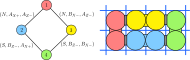
\includegraphics[width=\textwidth]{figures/topology_example.pdf}
    \caption{Example of a topology (left) for a system of the universal modules
    (right). Connection are denoted by gray rectangles, the naming of the docks
    follow figure \ref{fig:um_docks}. }
    \label{fig:topology_example}
\end{figure}

\paragraph{configuration} Intuitively, configuration is a topology with the
 module joints positions. Formally, a configuration $\mathcal{C}$ is a pair $(T,
 L)$:
 \begin{itemize}
    \item $T$ is a topology and
    \item $L: M \rightarrow \text{A} \rightarrow \mathds{R}$, where $A$ is a
    union of axis from all module types, is a function assigning values to all
    joints in the system.
 \end{itemize}

We define a \emph{model of a topology} $\mathcal{M}_\mathcal{T}$ as a descriptor
obtained by the following procedure:
\begin{enumerate*}
    \item rename uniquely descriptors of each module instance in the system, then
    \item select an arbitrary one and
    \item union the selected descriptor consequently with the other modules
    using module union (defined in section \ref{sec:capabilities}).
\end{enumerate*}
We define a \emph{model} $\mathcal{M}_\mathcal{C}$ of an configuration
$C=(T, L)$ as a model of $T$, where are labels were evaluated according to $L$,
i.e., labels are constant values. Configuration $C$ is \emph{realizable} iff:
\begin{enumerate*}
    \item for all pair of shoes, all paths in the model of $C$ yield the same
    relative position and
    \item no two shoes in the model of $C$ intersect.
\end{enumerate*}

There are no constraints on topology; therefore, we consider every topology
valid. However, for some topologies there exists no realizable configuration.
Given the terminology, there are few aspects to note:
\begin{itemize}
    \item To move the robot means to change a configuration.
    \item Change in configuration can also mean change in topology.
    \item Change in topology always means a change of configuration.
\end{itemize}

